\section{Conclusion}

\begin{frame}
    \tableofcontents[currentsection]
\end{frame}

\begin{frame}{Conclusion}
\begin{columns}
    \begin{column}{6cm}
    \centering{\textbf{Diagramme de Voronoï}}
    \begin{itemize}
        \item Plus lent en général pour le précalcul mais plus résistant aux grandes précisions
        \item Résultat satisfaisant même à basse précision !
        \item Chemin instantané
        \item Trajectoires plus satisfaisantes
        \item Plus adaptatif à la géométrie du problème
    \end{itemize}
    \end{column}
    \begin{column}{6cm}
    \centering{\textbf{Méthode naïve}}
    \begin{itemize}
        \item Rapide pour de faibles précisions, mais le résultat n'est pas toujours satisfaisant dans ce cas
        \item Très dépendant de la marge voulue par rapport aux obstacles
        \item Convient pour la géométrie très particulière de \textit{Micromouse}
    \end{itemize}
    \end{column}
\end{columns}
\end{frame}

% \begin{frame}
% \begin{figure}
%     \centering
%     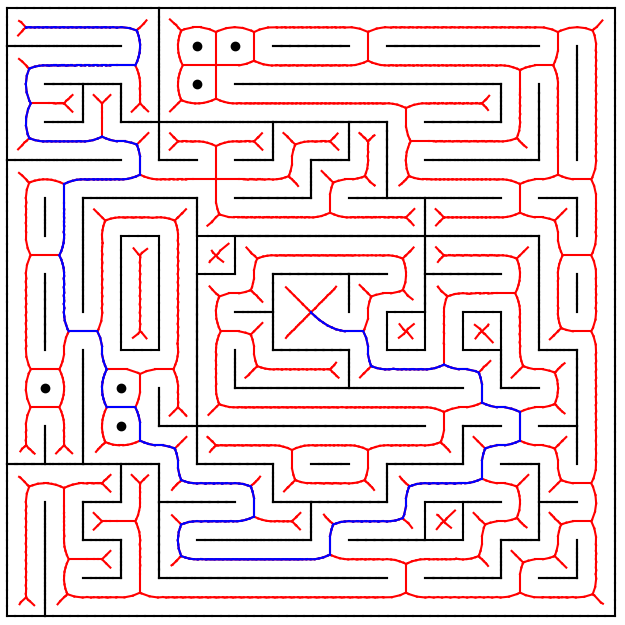
\includegraphics[width=0.7\linewidth]{assets/BigLabyrinthe.png}
% \end{figure}    
% \end{frame}